\section{Linguistische Theorien}

\begin{frame}
  {Ein neues semiotisches Dreieck}
  \onslide<+->
  \onslide<+->
  Im Sinn der letzten Woche interessiert uns nur die linke Seite.\\
  \onslide<+->
  \Zeile
  \centering 
  \begin{forest}
    [\gruen{Formen}
      [\gruen{Reale Objekte}, edge=gruen]
      [Mentale Konzepte]
    ]
  \end{forest}
\end{frame}

\begin{frame}
  {"`Semantik"' im generativen T-Modell}
  \onslide<+->
  \onslide<+->
  \centering 
  \resizebox{0.6\textwidth}{!}{
    \begin{tikzpicture}

      \node [rectangle, draw, align=left, color=teal, rounded corners=0.5em] (Numeration) at (5cm, -6cm) {Numeration};
      
      \node [visible on=<3->, rectangle, draw, align=left, color=gray] (Lexikon) at (1cm, -6cm) {Lexikon};
      \path (Lexikon.east) edge [visible on=<3->, line width=0.5mm, dashed] node [below, shift={(-0.4cm,0)}] {\textit{}} (Numeration.west);
     
      \node [visible on=<4->, rectangle, draw, align=left, color=gray] (Intention) at (9cm, -6cm) {Intention};
      \path (Intention.west) edge [visible on=<4->, line width=0.5mm, dashed] node [below, shift={(-0.4cm,0)}] {\textit{}} (Numeration.east);

      \node [visible on=<5->, rectangle, draw, align=left, fill=black, color=black, rounded corners=0.5em] (Syntax) at (5cm, -4.5cm) {\whyte{Syntax}};
      \path (Numeration.north) edge [visible on=<5->, line width=0.5mm, -latex] node [below, shift={(-0.4cm,0)}] {\textit{}} (Syntax.south);  

      \node [visible on=<6->, rectangle, draw, align=left, color=teal, rounded corners=0.5em] (Phrasenstruktur) at (5cm, -3cm) {Phrasenstruktur};
      \path (Syntax.north) edge [visible on=<6->, line width=0.5mm, -latex] node [below, shift={(-0.4cm,0)}] {\textit{}} (Phrasenstruktur.south);  

      \node [visible on=<7->, rectangle, draw, align=left, color=teal, rounded corners=0.5em] (PF) at (4cm, 0cm) {PF};
      \path (Phrasenstruktur.north) edge [visible on=<7->, line width=0.5mm, -latex] node [below, shift={(-0.4cm,0)}] {\textit{}} (PF.south);  
     
      \node [visible on=<8->, rectangle, draw, align=left, color=gray] (Aeusserung) at (1cm, 0cm) {Äußerung};
      \path (Aeusserung.east) edge [visible on=<8->, line width=0.5mm, dashed] node [below, shift={(-0.4cm,0)}] {\textit{}} (PF.west);
     
      \node [visible on=<9->, rectangle, draw, align=left, fill=black, color=black, rounded corners=0.5em] (Syntax2) at (6cm, -1.5cm) {\whyte{Syntax 2}};
      \path (Phrasenstruktur.north) edge [visible on=<9->, line width=0.5mm, -latex] node [below, shift={(-0.4cm,0)}] {\textit{}} (Syntax2.south);  
     
      \node [visible on=<10->, rectangle, draw, align=left, color=teal, rounded corners=0.5em] (LF) at (6cm, 0cm) {LF};
      \path (Syntax2.north) edge [visible on=<10->, line width=0.5mm, -latex] node [below, shift={(-0.4cm,0)}] {\textit{}} (LF.south);  

      \node [visible on=<11->, rectangle, draw, align=left, color=gray] (Interpretation) at (9cm, 0cm) {Interpretation};
      \path (Interpretation.west) edge [visible on=<11->, line width=0.5mm, dashed] node [below, shift={(-0.4cm,0)}] {\textit{}} (LF.east);
      
    \end{tikzpicture}
  }
\end{frame}

\begin{frame}
  {Repräsentationsebenen}
  \onslide<+->
  \onslide<+->
  Im klassischen generativen Modell:\\
  \grau{\footnotesize (In minimalistischen Modellen herrscht -- Chomsky muss es mögen! -- sowieso Anarchie.)}
  \Zeile
  \begin{itemize}[<+->]
    \item keine echte Interpretation auf LF
    \item Bewegung \rot{nachdem} der Satz geäußert wurde
    \item Herstellung einer logisch interpretierbaren \alert{Form} auf LF
    \item Grund | Syntax kann nicht alle Interpretationen abbilden
      \Halbzeile
      \begin{itemize}[<+->]
        \item[ ] \alert{Klassiker Quantorenskopus}
        \item[ ] \textit{Everybody loves somebody.}
          \Viertelzeile
        \item[A] Für alle Personen y gilt, dass es eine Person x gibt, für die gilt: y liebt x \grau{($\forall y\exists x.L(y,x)$)}
        \item[B] Es gibt eine Person x, sodass für alle Personen y gilt: y liebt x \grau{($\exists x\forall y.L(y,x)$)}
      \end{itemize}
  \end{itemize}
\end{frame}


\begin{frame}
  {Montagues direkte Interpretation}
  \onslide<+->
  \onslide<+->
  Sprache ist Logik ist Sprache \ldots\\
  \Halbzeile
  \begin{itemize}[<+->]
    \item[A] Entweder ist die \alert{Übersetzung in eine LF trivial und äquivalent zur PF\slash Syntax},\\
      oder \orongsch{sie fügt etwas hinzu, dass der Sprache an sich fehlt}.
    \item[B] Sätze haben aber auch \alert{mit LF-Übersetzung nur die Bedeutungen,\\
      die sie sowieso haben} \grau{(keine Hinzufügung)}.
    \item[\ding{222}] Also ist die \gruen{Übersetzung in LF trivial und äquivalent zur PF\slash Syntax}.
    \item[\ding{222}] Wir können \gruen{Sätze direkt interpretieren} (wie sie gesprochen\slash geschrieben werden).
     \Zeile 
   \item \alert{Montagues \textit{lf}} | direkte Übersetzung von sprachlichen in logische Ausdrücke
  \end{itemize}
\end{frame}

\section{Referentielle Semantik basal}

\begin{frame}
  {Interessante Eigenschaften von Sprache}
  \onslide<+->
  \begin{itemize}[<+->]
    \item Aussagen über die\slash Teile der Welt
    \item Ausdrücke bezeichnen\slash referieren auf Dinge i.\,w.\,S.
    \item Informativität
    \item objektiv beurteilbar (\zB Wahrheit von Sätzen)
      \Zeile
    \item \alert{Aber welche sprachlichen Einheiten referieren auf was?}
  \end{itemize}
\end{frame}

\begin{frame}
  {Referenz | Eigennamen}
  \onslide<+->
  \onslide<+->
  Ein \alert{Eigenname} \ding{222} \alert{genau ein Objekt} in der Welt\\
  \onslide<+->
  \Zeile
  \centering
    \begin{tikzpicture}
      \node [] (name) at (-6cm, 0cm) {\textit{Jan Böhmermann}};
      \node [visible on=<4->] (boehmi) at (0cm, 0cm) {\includegraphics[width=0.2\textwidth]{\GRAPHPATH/boehmermann}};
      \path (name.east) edge [visible on=<4->, line width=0.5mm, -latex] node {\textit{}} (boehmi.west);
    \end{tikzpicture}
\end{frame}

\begin{frame}
  {Referenz | Appellativa}
  \onslide<+->
  \onslide<+->
  Ein normales \alert{Nomen} \ding{222} \alert{eine Menge von Objekten} in der Welt\\
  \onslide<+->
  \Zeile
  \centering
    \begin{tikzpicture}
      \node [] (noun) at (-6cm, 0cm) {\textit{soldier}};
      \node [visible on=<4->] (soldiers) at (0cm, 0cm) {
\includegraphics[width=0.2\textwidth]{\GRAPHPATH/soldiers}};
      \path (noun.east) edge [visible on=<4->, line width=0.5mm, -latex] node {\textit{}} (soldiers.west);
    \end{tikzpicture}
\end{frame}

\begin{frame}
  {Referenz | Adjektive und Verben}
  \onslide<+->
  \onslide<+->
  Ein (intersektives) \alert{Adjektiv} oder ein \alert{Verb} \ding{222} \alert{eine Menge von Objekten} in der Welt\\
  \onslide<+->
  \Zeile
  \centering
    \begin{tikzpicture}
      \node [] (adj) at (-6cm, 0cm) {\textit{human}};
      \node [visible on=<4->] (boehmi) at (0cm, +2cm) {\includegraphics[width=0.1\textwidth]{\GRAPHPATH/boehmermann}};
      \path (adj.east) edge [visible on=<4->, line width=0.5mm, -latex] node {\textit{}} (boehmi.west);
      \node [visible on=<5->] (soldiers) at (0cm, 0cm) {
\includegraphics[width=0.1\textwidth]{\GRAPHPATH/soldiers}};
      \path (adj.east) edge [visible on=<5->, line width=0.5mm, -latex] node {\textit{}} (soldiers.west);
      \node [visible on=<6->] (crowd) at (0cm, -2cm) {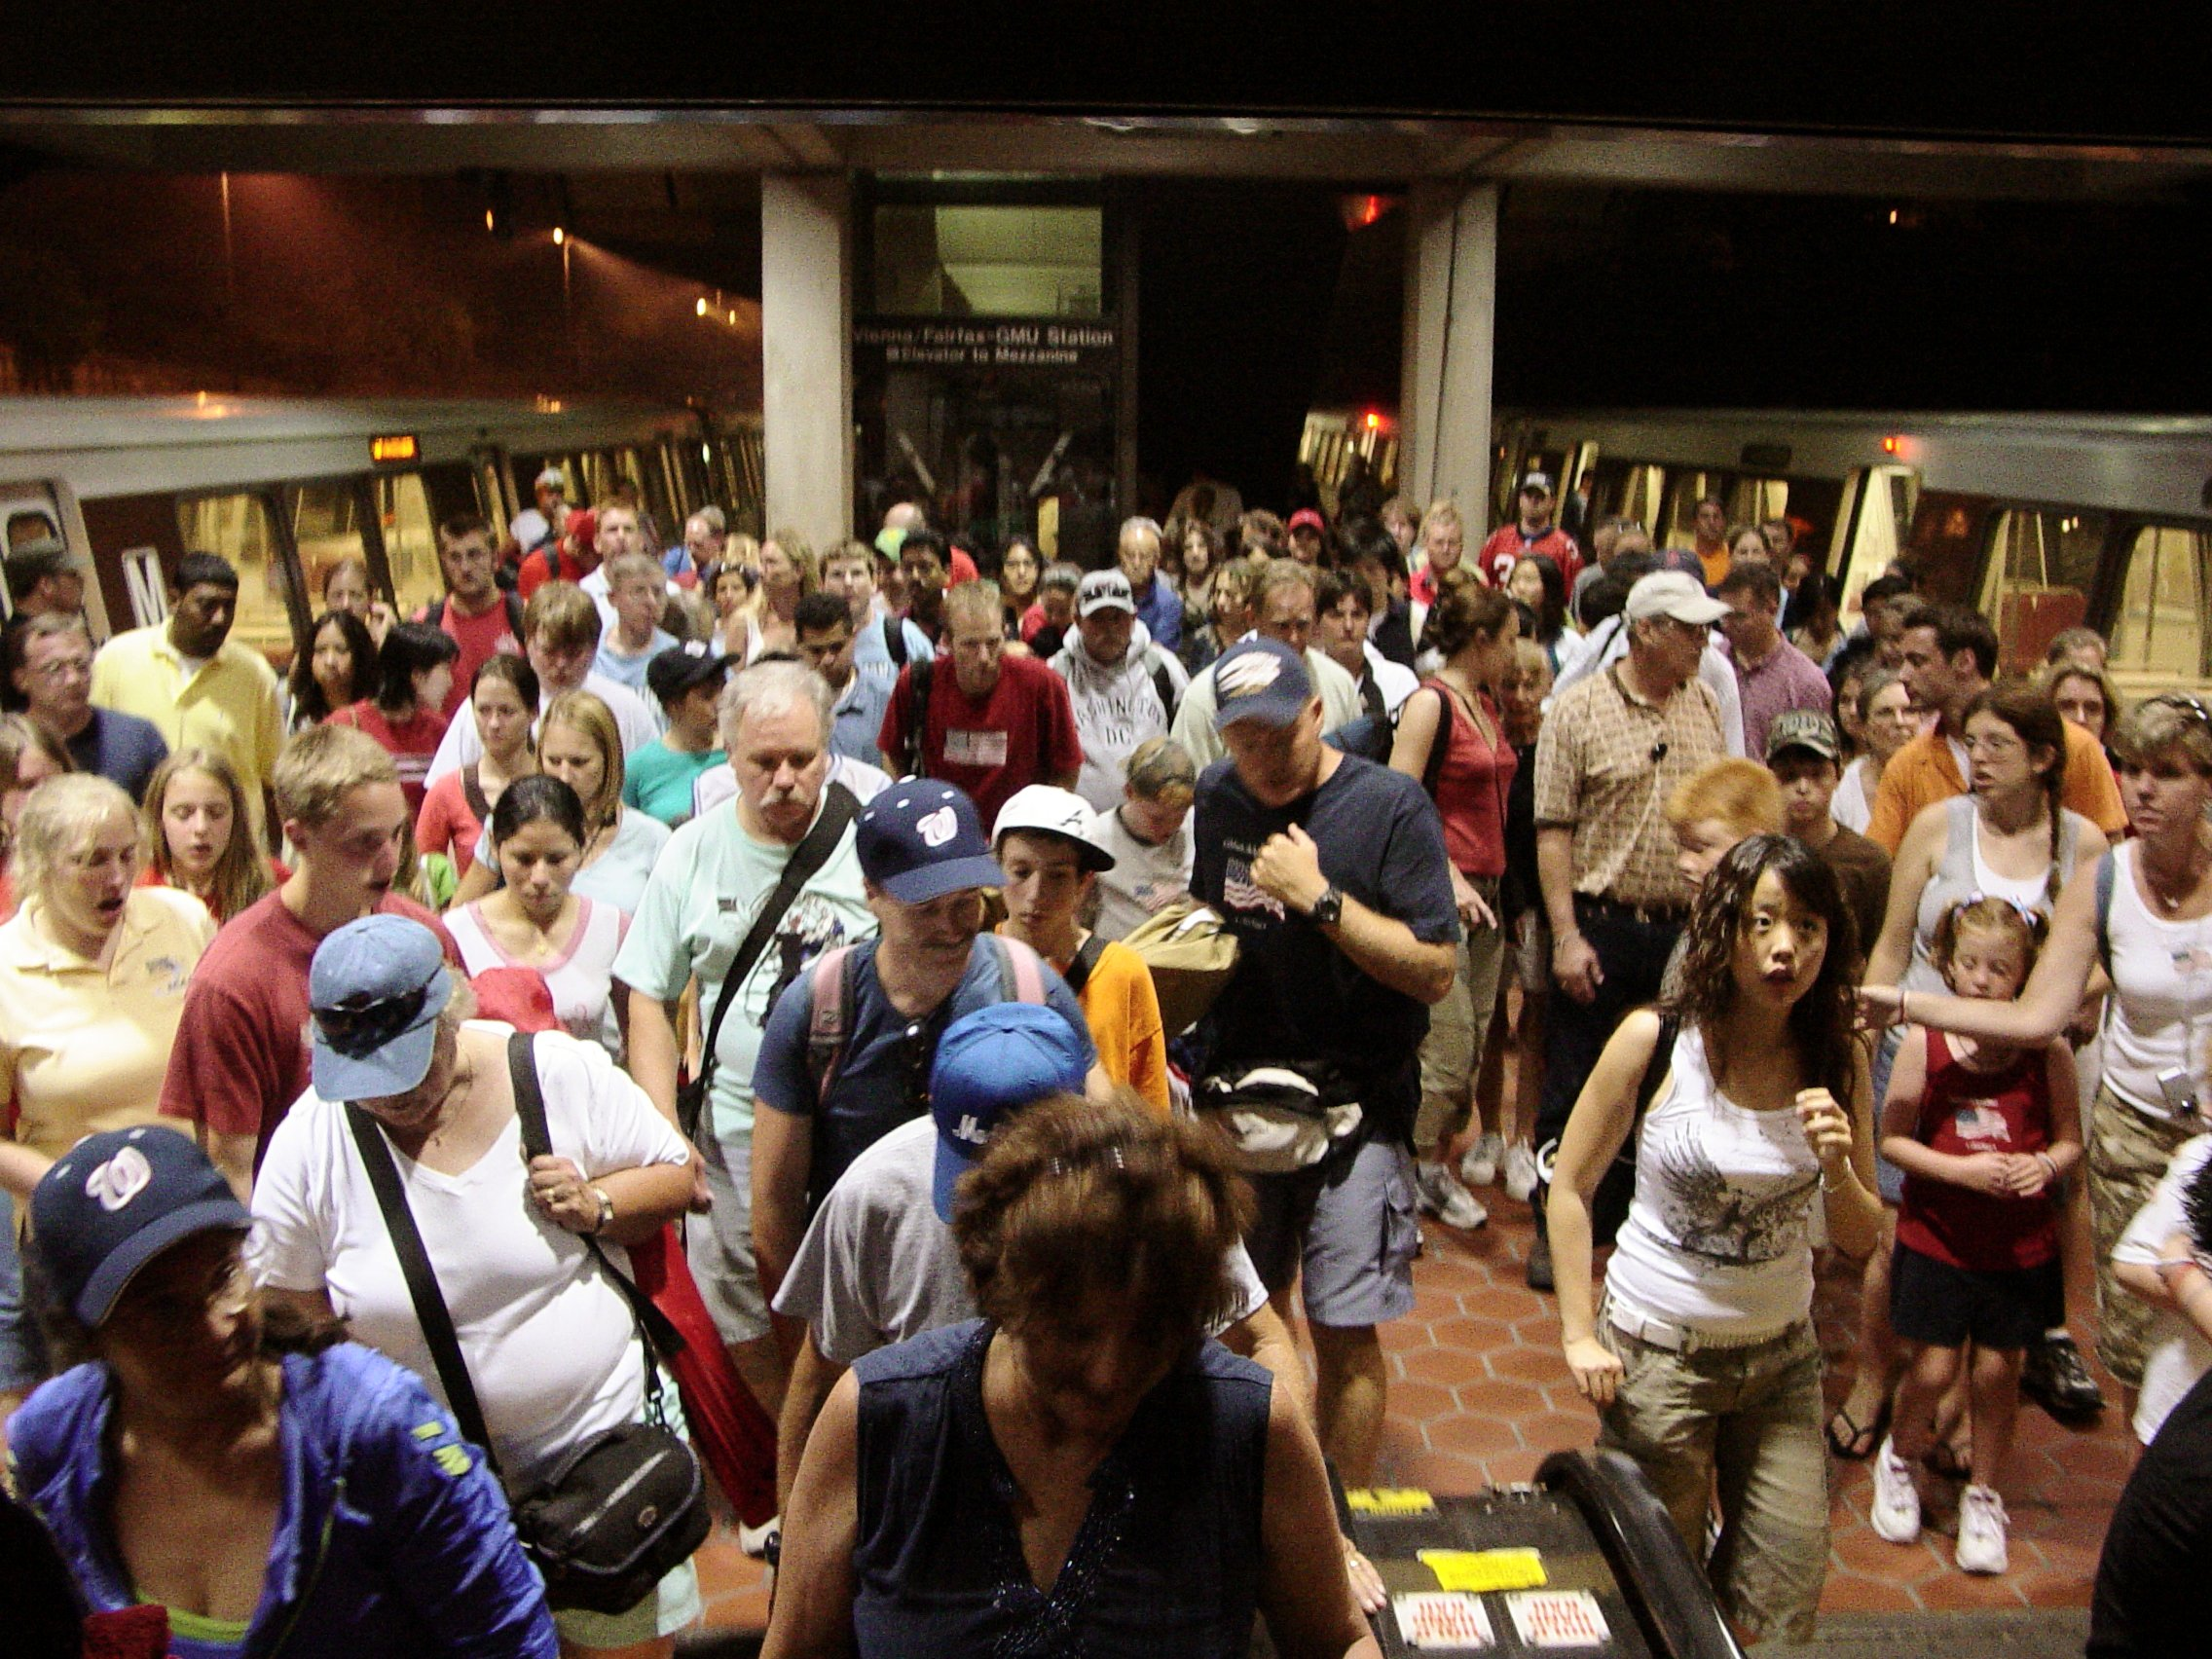
\includegraphics[width=0.1\textwidth]{\GRAPHPATH/crowd}};
      \path (adj.east) edge [visible on=<6->, line width=0.5mm, -latex] node {\textit{}} (crowd.west);
    \end{tikzpicture}
\end{frame}

\begin{frame}
  {Referenz | Sätze}
  \onslide<+->
  \onslide<+->
  Ein \alert{Satz} \ding{222} in erster Näherung \alert{ein Sachverhalt}\\
  \onslide<+->
  \Zeile
  \centering
    \begin{tikzpicture}
      \node [align=left] (s) at (-6cm, 0cm) {\it A humming bird\\\it is hovering over\\\it a red flower.};

      \node [visible on=<4->, align=center] (hum) at (0cm, +2cm) {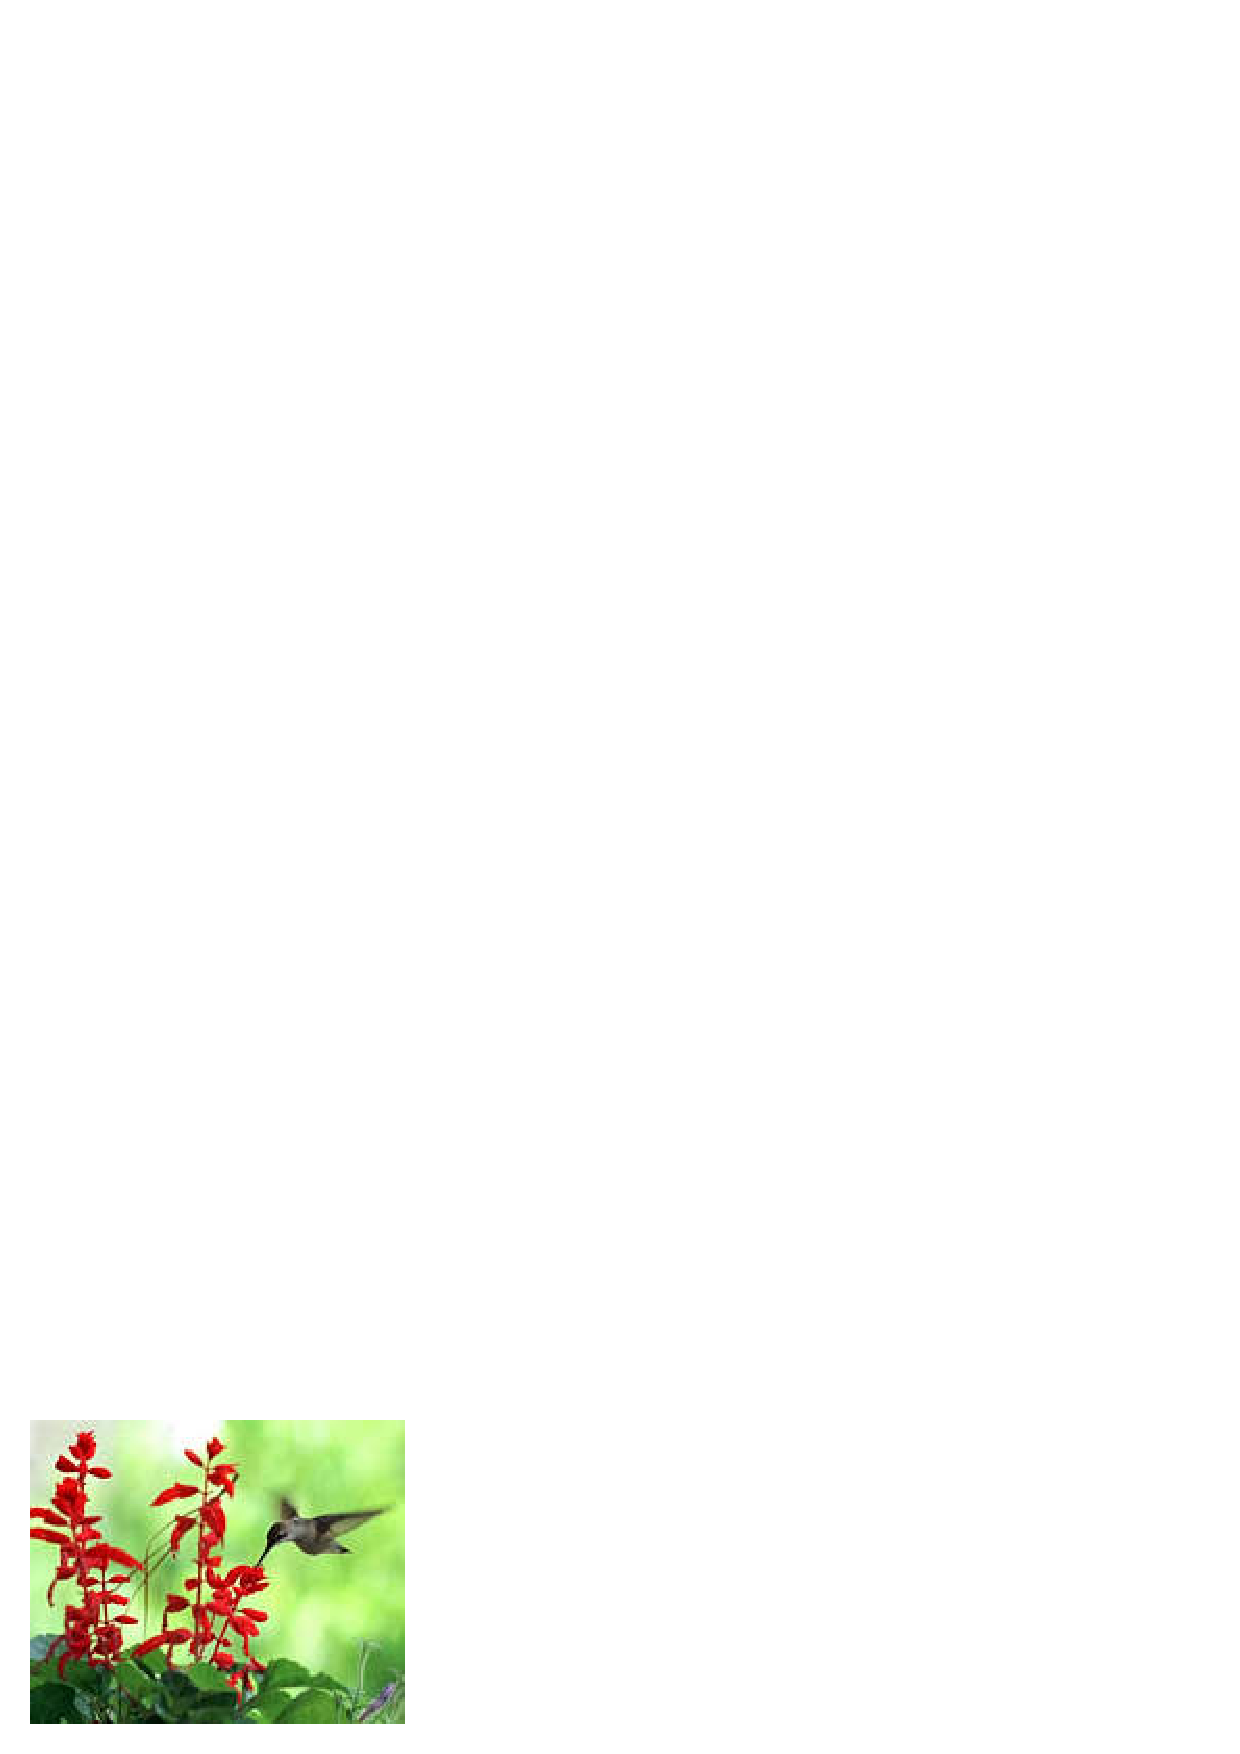
\includegraphics[width=0.2\textwidth]{\GRAPHPATH/hummingbird}};
      \path (s.east) edge [visible on=<4->, line width=0.5mm, -latex] node {\textit{}} (hum.west);
      
      \node [visible on=<5->, align=center] (boehmi) at (0cm, -2cm) {\includegraphics[width=0.2\textwidth]{\GRAPHPATH/boehmermann}\\\footnotesize (als Individuum)};
      \path (s.east) edge [visible on=<5->, line width=0.5mm, -latex, color=red] node {\textit{}} (boehmi.west);
      \node [visible on=<6->, align=center, color=red, fill=red] (nein) at (-3.5cm, -1.25cm) {\footnotesize \whyte{Nein! falsche}\\\footnotesize \whyte{Art von Objekt}};
    \end{tikzpicture}
\end{frame}

\begin{frame}
  {Freges Prinzip | Das hier wollen wir formalisieren!}
  \onslide<+->
  \onslide<+->
  Bedeutung ist kompositional!\\
  \Halbzeile
  \begin{itemize}[<+->]\small
    \item \textit{humming bird} \ding{222} die \alert{Menge} der Kolibri-Objekte
    \item \textit{a} \ding{222} \alert{Existenzaussage} für ein Element aus einer Menge
    \item \textit{a humming bird} \ding{222} \alert{Existenzaussage} für ein Element $x$\\
      aus der Menge der Kolibri-Objekte
    \item \textit{is hovering} \ding{222} die \alert{Menge} der schwebenden Objekten
    \item \textit{a humming bird is hovering} \ding{222} das existierende Kolibri-Objekt $x$\\
      ist auch ein \alert{Element der Menge} der schwebenden Objekte
    \item \textit{a red flower} \ding{222} \alert{Existenzaussage} für ein Element $y$\\
      aus der \alert{Schnittmenge} der roten Objekte und der Blumen-Objekte
    \item \textit{over} \ding{222} die \alert{Relation} zwischen Objekten (s.\ nächste Woche),\\
      die sich übereinander befinden
    \item \textit{A Humming is hovering over a red flower.} \ding{222}\\
      \gruen{Es gibt ein Objekt $x$ aus der Schnittmenge der Kolibri- und der schwebenden Objekte,\\
      und es gibt ein Objekt $y$ aus der Schnittmenge der roten und der Blumen-Objekte,\\
    und $x$ befindet sich über $y$.}
  \end{itemize}
\end{frame}

\section{Semantische Eigenschaften von Sätzen}

\begin{frame}
  {Implikation (Entailment)}
  \onslide<+->
  \onslide<+->
  Mengen von Aussagesätzen \alert{implizieren} andere Sätze.\\
  \onslide<+->
  Sätze (Implikationen) lassen sich aus anderen Sätzen (Axiome) \alert{beweisen}.\\
  \Halbzeile
  \begin{itemize}[<+->]
    \item[A] \textit{Jan Böhmermann ist ein Mensch.}
    \item[B] \textit{Jan Böhmermann ist leutselig.}
    \item[C] \textit{Jan Böhmermann ist ein leutseliger Mensch.}
      \Halbzeile
    \item[ ] \alert{$A,B\vdash C$} | A und B implizieren C. (C ist beweisbar aus A und B.)
    \item[ ] \rot{$A\not\vdash C$} | A impliziert nicht C.
    \item[ ] \rot{$B\not\vdash C$} | B impliziert nicht C.
      \Halbzeile
    \item[ ] \orongsch{$A\vdash A\wedge A$} \onslide<+->| \textit{Jan Böhmermann ist ein Mensch \orongsch{und} Jan Böhmermann ist ein Mensch.}
      \Halbzeile
    \item[D] \textit{Irgendetwas ist ein Mensch.}
    \item[ ] \alert{$A\vdash D$} 
  \end{itemize}
\end{frame}

\begin{frame}
  {Tests auf Implikation}
  \onslide<+->
  \onslide<+->
  Wenn diese Kriterien zutreffen, impliziert A B:\\
  \Zeile
  \begin{itemize}[<+->]
    \item Wenn A wahr ist, ist B auch immer wahr.
    \item Eine Situation, die von B beschrieben wird, wird auch von A beschrieben.
    \item Die Information in B ist vollständig in der Information in A enthalten.
    \item Man kann unter keinen Umständen sagen: \textit{A ist wahr, aber B ist nicht wahr.}
  \end{itemize}
\end{frame}

\begin{frame}
  {Übung | Sind das Implikationen?}
  \begin{itemize}[<+->]\small
    \item Böhmermann ist Showmaster. $\vdash$ Böhmermann ist menschlich.
    \item Böhmermann ist nicht sehr groß. $\vdash$ Irgendjemand ist nicht sehr groß.
    \item Böhmermann ist nicht sehr groß. $\vdash$ Irgendjemand ist sehr groß.
    \item Manche Menschen sind leutselig. $\vdash$ Böhmermann ist leutselig.
    \item Ich habe das neue drip-133-Album gehört. $\vdash$ drip-133 hat ein neues Album veröffentlicht.
    \item Nachdem ich einen Sherry getrunken habe, habe ich den Kondensator getauscht.\\
      $\vdash$ Ich habe einen Sherry getrunken.
    \item Nachdem Linux nicht mehr startete, habe ich einen weiteren Sherry getrunken.\\
      $\vdash$ Linux ist noch nie gestartet.
    \item Mein ehemaliger Mitbewohner mag Becks.\\
      $\vdash$ Mein ehemaliger Mitbewohner könnte Sherry mögen.
    \item Böhmermann hat das heutige ZDF Magazin beendet.\\
      $\vdash$ Das heutige ZDF Magazin wurde beendet.
  \end{itemize}
\end{frame}

\begin{frame}
  {Präsupposition | Der plausible HIntergrund}
  \onslide<+->
  \onslide<+->
  Präsuppositionen sind schwächer als Implikationen.\\
  \Zeile
  \begin{itemize}[<+->]
    \item[A] \textit{Willy Brandt ist der gegenwärtige Kanzler Deutschlands.}
    \item[B] \textit{Wenn Willy Brandt der gegenwärtige Kanzler Deutschlands ist,\\
      trägt er eine große Verantwortung.}
    \item[C] \textit{Willy Brandt ist nicht der gegenwärtige Kanzler Deutschlands.}
    \item[D] \textit{Willy Brandt lebt.}
    \item[E] \textit{Es gibt einen Kanzler Deutschlands.}
      \Halbzeile
    \item \alert{A und B präsupponieren D.} = D ist eine Voraussetzung\\
      für eine erfolgreiche Interpretation von A und B.
    \item \orongsch{C präsupponiert nicht D.}
    \item \alert{A, B und C präsupponieren E.}
      \Halbzeile
    \item Die einzige Implikation hier: $A\vdash E$
  \end{itemize}
\end{frame}

\begin{frame}
  {Tests auf Präsupposition}
  \onslide<+->
  \onslide<+->
  Die Unterschiede zur Implikation sind relevant.\\
  \Halbzeile
  \begin{itemize}[<+->]
    \item Nicht nur Aussagesätzen haben Präsuppositionen (Modale, Konditionale, \ldots)
    \item Negierte Sätze haben oft gleiche Präsuppositionen wie nicht-negierte.
    \item Präsuppositionen können negiert werden, und der Ausgangssatz bleibt wahr.\\
      \grau{(Geht nicht mit Implikationen.)}
      \begin{itemize}[<+->]
        \item[F] \textit{Willy Brandt ist nicht Kanzler Deutschlands.}
        \item[G] \textit{Es gibt einen Kanzler Deutschlands.}
        \item[ ] F präsupponiert G, bleibt aber wahr, wenn G falsch ist.
      \end{itemize}
  \end{itemize}
\end{frame}

\begin{frame}
  {Synonymie}
  \onslide<+->
  \onslide<+->
  Synonyme Ausdrücke haben \orongsch{exakt} \alert{die gleiche Referenz}.\\
  \Halbzeile
  \begin{itemize}[<+->]
    \item lexikalische Synonymie | \textit{humming bird} $\stackrel{lex}{\equiv}$ \textit{colibri}
      \Halbzeile
    \item kompositionale Synonymie
      \begin{itemize}[<+->]
        \item[ ] \textit{Mulder traf seine entführte Schwester, nachdem er\\
          in die geheime Militärbasis eingebrochen war.}
        \item[$\equiv$] \textit{Bevor er seine entführte Schwester traf, brach Mulder in die geheime Militärbasis ein.}
      \end{itemize}
    \Halbzeile
    \item \alert{$A\equiv B\ \text{gdw}\ A\vdash B\ \text{und}\ B\vdash A$} (gegenseitige Implikation)
    \item \grau{\textit{gdw} = \textit{genau dann wenn} | \textit{iff} = \textit{if and only if}}
  \end{itemize}
\end{frame}

\section{Referenz von Sätzen}

% \subsection{Referential and non-referential NPs}
% \frame{\frametitle{Noun-like expressions and complex NPs}
%  \begin{itemize}
%    \item<1-> I saw \textcolor{blue}{a man}.
%    \item<2-> I saw \textcolor{blue}{the green wobbly thing crawling near}.
%    \item<3-> I saw \textcolor{blue}{it}.
%  \end{itemize}
% }
% 
% \frame{\frametitle{Problems with referential NPs}
%  \begin{itemize}
%    \item<1-> \emph{\textcolor{blue}{The dark subatomic particles in the universe} have a total mass much larger than the visible subatomic particles.}
%    \item<2-> \emph{\textcolor{blue}{Problems with referential semantic theories} don't concern \textcolor{blue}{Rumpletweezer}.}
%    \item<3-> \textcolor{red}{and of course, vagueness (e.g., Sorites Paradox)}
%  \end{itemize}
% }
% 
% \frame{\frametitle{Problems with non-referential NPs}
%  \begin{itemize}
%    \item<1-> \emph{some guy}
% 	 \item<2-> \emph{not the faintest trace of blood}
% 	 \item<3-> \emph{any axiom of Zermelo-Fraenkel set theory}
%  \end{itemize}
% }

\begin{frame}
  {Natürliche Sprache und Implikation}
  \onslide<+->
  \onslide<+->
  Referentielle Semantik $\not=$ \alert{\textit{Zeigen auf Objekte durch Sprache}}.\\
  \Viertelzeile
  \onslide<+->
  Zusätzliche Logik für Fälle wie diesen (und viele andere):\\
  \Zeile
  \onslide<+->
  \begin{tabular}[h]{lll}
    & \alert{\textit{Die Lieblingsblume meines Kolibris}} & \textit{ist rot.} \\
    \visible<6->{\orongsch{$\vdash$}} & \visible<5->{\alert{\textit{Eine Blume}} & \textit{ist rot.}} \\
  \end{tabular}
\end{frame}

\begin{frame}
  {Sätze referieren aus Wahrheitswerte!}
  \onslide<+->
  \onslide<+->
  \centering 
  Um zu der gewünschten Logik zu kommen, zeigen wir jetzt,\\
  dass \alert{Sätze auf Wahrheitswerte referieren}.\\
  \Halbzeile
  \onslide<+->
  Wahrheitswerte sind nur \alert{\textit{wahr}} und \alert{\textit{falsch}}.\\
  \Halbzeile
  \onslide<+->
  Die Verben \alert{\textit{denotieren}} und \textit{\alert{referieren auf}} sind hier synonym.\\
  \Doppelzeile
  \onslide<+->
  Warten Sie bitte ein paar Wochen, wenn Sie diese Darstellung reduktionistisch finden.
\end{frame}

\begin{frame}
  {Synonyme NPs}
  \onslide<+->
  \begin{itemize}[<+->]
    \item[a] \textit{colibri}
    \item[b] \textit{humming bird}
    \item[ ] \gruen{$a\stackrel{lex}{\equiv} b$}
      \Halbzeile
    \item[c] \textit{a brunette lady}
    \item[d] \textit{a brown-haired dame}
    \item[ ] \gruen{$c\equiv d$}
      \Halbzeile
    \item[e] \textit{the primates}
    \item[f] \textit{the apes and humans}
    \item[ ] \gruen{$e\equiv f$}
  \end{itemize}
\end{frame}

\begin{frame}
  {Synonymie von Konstituenten und Sätzen}
  Synonymie von Konstituenten im Satzkontext \ding{222} Satzsynonymie\\
  \onslide<+->
  \Halbzeile
  \begin{itemize}[<+->]
    \item[A] \alert{\textit{A \orongsch{colibri} is hovering over a red flower.}}
    \item[B] \alert{\textit{A \orongsch{humming bird} is hovering over a red flower.}}
    \item[ ] \gruen{$A\equiv B$ weil $a\equiv b$ und Satzkontext identisch}
      \Halbzeile
    \item[C] \alert{\textit{Lauren Bacall was \orongsch{a brunette lady}.}}
    \item[D] \alert{\textit{Lauren Bacall was \orongsch{a brown-haired dame}.}}
    \item[ ] \gruen{$C\equiv D$ weil $c\equiv d$ und Satzkontext identisch}
      \Halbzeile
    \item[E] \alert{\textit{\orongsch{Primates} are intelligent.}}
    \item[F] \alert{\textit{\orongsch{The apes and humans} are intelligent.}}
    \item[ ] \gruen{$E\equiv F$ weil $e\equiv f$ und Satzkontext identisch}
  \end{itemize}
\end{frame}

\begin{frame}
  {Zwei Axiome}
  \onslide<+->
  \begin{itemize}[<+->]
    \item[ ] Referenz\slash Denotat eines Ausdrucks A: \alert{\den{A}}
      \Zeile
    \item[ ] Erinnerung: Synonymität für Sätze ist gegenseitige Implikation.
      \Zeile
    \item[Ax1] Synonyme Ausdrücke (NPs, Verben, Sätze, \ldots) haben dieselbe Referenz.
    \item[ ] Formal: \alert{$A\equiv B\leftrightarrow\den{A}=\den{B}$}
      \Zeile
    \item[Ax2] Wenn wir in Ausdruck C einen Ausdruck A durch\\
      einen synonymen Ausdruck B ersetzen, behält C seine Referenz.
    \item[ ] Formal: \alert{$\den{A}=\den{B}\rightarrow\den{[\Sub{C} A]}=\den{[\Sub{C} B]}$}
  \end{itemize}
\end{frame}

\begin{frame}
  {Zwei wahre Sätze}
  \onslide<+->
  \onslide<+->
  Wahrheitswert von A und B | 1 bzw.\ \textit{wahr}\\
  \onslide<+->
  \Zeile
  \begin{itemize}[<+->]
    \item[A] \textit{Lauren Bacall was a brunette lady.}
    \item[B] \textit{My humming bird's favourite flower is red.} 
  \end{itemize}
\end{frame}

\begin{frame}
  {Erste Schlussfolgerung}
  \onslide<+->
  \onslide<+->
  Einsetzen von A und B in Satz T (Aussage über Wahrheitswert)\\
  \Halbzeile
  \begin{itemize}[<+->]
    \item[T] \alert{\textit{The truth value of `\_\_\_' is 1.}}
      \Halbzeile
    \item[{[\Sub{T}A]}] \alert{\textit{The truth value of `\orongsch{Lauren Bacall was a brunette lady.}' is 1.}}
    \item[{[\Sub{T}B]}] \alert{\textit{The truth value of `\orongsch{My humming bird's favourite flower is red.}' is 1.}}
      \Halbzeile
    \item[ ] folgt \gruen{$A\equiv[\Sub{T}A]$} und \gruen{$B\equiv[\Sub{T}B]$}
    \item[ ] mit Ax1 \gruen{$\den{A}=\den{[\Sub{T}A]}$} und \gruen{$\den{B}=\den{[\Sub{T}B]}$}
      \Halbzeile
    \item[ ] Bitte bedenken: $A$ und $[\Sub{T}A]$ haben auch intuitiv "`dieselbe Aussage"'.
  \end{itemize}
\end{frame}

\begin{frame}
  {Zweite Schlussforlgerung}
  \onslide<+->
  \onslide<+->
  In $[\Sub{T}A]$ und $[\Sub{T}B]$ sind A und B jeweils in einer NP eingebettet.\\
  \Halbzeile
  \begin{itemize}[<+->]
    \item $\den{the truth value of A}=\den{the truth value of B}=1$
    \item[ ] mit Ax2 \gruen{$\den{[\Sub{T}A]}=\den{[\Sub{T}B]}$}
    \item[ ] damit \gruen{$\den{A}=\den{[\Sub{T}A]}=\den{[\Sub{T}B]}=\den{B}=1$}
      \Halbzeile
    \item \gruen{Sätze referieren auf Wahrheitswerte.}\\
      \grau{(Denn man kann das mit zwei beliebigen wahren Sätzen machen.)}
  \end{itemize}
\end{frame}

\frame{\frametitle{Advantages of truth values}
\begin{itemize}
  \item<1-> indirect encoding of `richer' semantics (One must know the truth conditions of a sentence and the state of affairs to decide about the truth of a sentence.)
  \item<2-> a minimal common semantic property of sentences
  \item<3-> easily computable in a formal system (binary)
  \item<4-> their logic provides a basis for `richer' semantics (cf. second half of class)
\end{itemize}
}

\subsection{Sense and reference}
\frame{\frametitle{Frege also thought, reference couldn't be all}
\begin{center}
\begin{tabular}{|l|l|l|}
  \hline
  \textbf{Type} & \textbf{Reference} & \textbf{Sense} \\
  \hline
  \hline
  NP & individuals & individual concepts \\
      & \emph{Venus} & \\
  \hline
  VP & sets & property concepts \\
  & \emph{humming birds} & \\
  \hline
  S & 1 or 0 & thoughts \\
  & \emph{I like cats.} & \\
  \hline
\end{tabular}
\end{center}
}

\frame{\frametitle{Some terminology}
\begin{itemize}
  \item<1-> \emph{reference} = \emph{extension}	= what we're dealing with first
  \item<2-> \emph{sense} = \emph{intension} = what we will be dealing with later
  \item<3-> \emph{proposition} = the intensions of sentences as informational content: The `thought that S'.
\end{itemize}
}

\section{We're talking in fragments: F1}
\frame{\frametitle{Decomposing compositionality and composing truth}
\begin{itemize}
 \item<1-> How are sentences compositionally built up? 
 \item<2-> What do their parts denote?
 \item<3-> How does the denotation of the parts contribute to the whole.
 \item<4-> T-sentences: \textcolor{blue}{S of L is true in v iff p.}
 \item<5-> {\footnotesize \emph{S} a sentence, \emph{L} a language, \emph{v} a state of affairs, \emph{p} a statement of the truth conditions.}
\end{itemize}
}

\subsection{A syntax}

\frame{\frametitle{A phrase-structure grammar}
\begin{itemize}
 \item<1-> S $\rightarrow$ N VP
 \item<2-> S $\rightarrow$ S conj S	
 \item<3-> S $\rightarrow$	neg S
 \item<4-> VP $\rightarrow$ V\Sub{{i}}
 \item<5-> VP $\rightarrow$ V\Sub{t} N
\end{itemize}
}

\frame{\frametitle{A lexicon}
\begin{itemize}
 \item<1-> N $\rightarrow$ \emph{Herr Webelhuth, Frau Eckardt, the Turm-Mensa}
 \item<1-> V\Sub{{i}} $\rightarrow$ \emph{is relaxed, is creative, is stupid}
 \item<1-> V\Sub{t} $\rightarrow$ \emph{prefers}
 \item<1-> conj $\rightarrow$ \emph{and, or}
 \item<1-> neg $\rightarrow$ \emph{it is not the case that}
\end{itemize}
}

\subsection{The semantics: individuals, sets, functions, T-sentences}
\frame{\frametitle{Simple denotiations}
\begin{itemize}
  \item<1-> $\llbracket$Herr Webelhuth$\rrbracket$ = Herr Webelhuth
  \item<2-> $\llbracket$Frau Eckardt$\rrbracket$ = Frau Eckardt
  \item<3-> $\llbracket$the Turm-Mensa$\rrbracket$ = the Turm-Mensa
  \item<4-> $\llbracket$is relaxed$\rrbracket$ = \{x:x is relaxed\}
  \item<5-> $\llbracket$is creative$\rrbracket$ = \{x:x is creative\}
  \item<6-> $\llbracket$is stupid$\rrbracket$ = \{x:x is stupid\}
  \item<7-> $\llbracket$prefers$\rrbracket$ = \{$\langle$x,y$\rangle$: x prefers y\}
\end{itemize}
}

\frame{\frametitle{Some words don't really `denote', they act like functions}
\begin{itemize}
  \item<1-> $\dem{neg} = \left[
                         \begin{array}{l}
	                          1 \rightarrow 0\\
	                          0 \rightarrow 1
                         \end{array}
                         \right]$
  \item<2-> $\dem{and} = \left[
                         \begin{array}{l}
	                          \langle 1,1 \rangle \rightarrow 1\\
	                          \langle 1,0 \rangle \rightarrow 0\\
	                          \langle 0,1 \rangle \rightarrow 0\\
	                          \langle 0,0 \rangle \rightarrow 0
                         \end{array}
                         \right]$
  \item<3-> $\dem{or} = \left[
                         \begin{array}{l}
	                          \langle 1,1 \rangle \rightarrow 1\\
	                          \langle 1,0 \rangle \rightarrow 1\\
	                          \langle 0,1 \rangle \rightarrow 1\\
	                          \langle 0,0 \rangle \rightarrow 0
                         \end{array}
                         \right]$
  \end{itemize}
}

\frame{\frametitle{T-sentences: rule-to-rule}
\begin{itemize}
  \item<1-> \den{[\Sub{S}{ }N{ }VP]} = 1 iff \den{N} $\in$ \den{VP}, else 0
  \item<2-> \den{[\Sub{S} S1 conj S2]} = \den{conj} ($\langle$\den{S1},\den{S2}$\rangle$)
  \item<3-> \den{[\Sub{S} neg S]} = \den{neg} (\den{S})
  \item<4-> \den{[\Sub{VP} V\Sub{t} N]} = \{x: $\langle$x, \den{N} $\rangle$ $\in$ \den{V\Sub{t}}\}
  \item<5-> semantics for non-branching nodes: \textcolor{blue}{pass-up}
\end{itemize}
}

\subsection{Bottom-up evaluation}
\frame{\frametitle{A starting point for our computation}
\textcolor{blue}{\emph{Herr Webelhuth is relaxed.}}\\

\begin{itemize}
  \item<1-> Circumstances (Model): Herr Webelhuth is an element of the set of relaxed individuals.\\{}
  \item<2-> (1) The syntax is well-formed by S $\rightarrow$ N VP
  \item<3-> (2) for N: \den{Herr Webelhuth} = Herr Webelhuth
  \item<4-> (3) for VP: \den{is relaxed} = \{x: x is relaxed\}
  \item<5-> (4) for S: \den{[\Sub{S}{ }N{ }VP]} = 1 iff \den{N} $\in$ \den{VP}, else 0
\end{itemize}
}

\frame{\frametitle{A starting point for our computation}
The tree:\\

\begin{center}
 \begin{bundle}
   {1 since \den{Herr Webelhuth} $\in$ \den{is relaxed}}
     \chunk[N]{\den{Herr Webelhuth}}
     \chunk[VP]{\den{is relaxed}}
 \end{bundle}
\end{center}
}

\frame{\frametitle{We compute syntactic representations, not flat sentences}
\emph{\textcolor{blue}{(\Sub{S1} Frau Eckardt is creative)} and it is not the case that \textcolor{green}{(\Sub{S2} Herr Webehlhuth is relaxed)} and \textcolor{red}{(\Sub{S3} Frau Eckardt prefers the Turm-Mensa)}.}\\
\begin{center}
\begin{tabular}{cc}
 \begin{bundle}
   {S}\setlength\GapDepth{2ex}\setlength\GapWidth{1em}
   \chunk{\textcolor{blue}{S\Sub{1}}}
     \chunk{conj}
     \chunk{
             \begin{bundle}
               {S}
               \chunk{neg}
               \chunk{\begin{bundle}
                         {S}
                         \chunk{\textcolor{green}{S\Sub{2}}}
                         \chunk{conj}
                         \chunk{\textcolor{red}{S\Sub{3}}}
                       \end{bundle}
                     }
             \end{bundle}        
           }
 \end{bundle} &
 \begin{bundle}
   {S}\setlength\GapDepth{2ex}\setlength\GapWidth{1em}
     \chunk{\textcolor{blue}{S\Sub{1}}}
     \chunk{conj}
     \chunk{
             \begin{bundle}
               {S}
               \chunk{\begin{bundle}
                       {S}
                       \chunk{neg}
                       \chunk{\textcolor{green}{S\Sub{2}}}
                      \end{bundle}
                     }
               \chunk{conj}
               \chunk{\textcolor{red}{S\Sub{3}}}
             \end{bundle}        
           }
 \end{bundle}  \\
\end{tabular}
\end{center}
}

\frame{\frametitle{A starting point for our computation}
Circumstances: Herr Webelhuth is relaxed, Frau Eckardt is creative, and Frau Eckardt does not prefer the Turm-Mensa:\\

\begin{center}
\begin{tabular}{cc}
 \begin{bundle}
   {1}\setlength\GapDepth{2ex}\setlength\GapWidth{1em}
     \chunk{\textcolor{blue}{1}}
     \chunk{conj}
     \chunk{
             \begin{bundle}
               {1}
               \chunk{neg}
               \chunk{\begin{bundle}
                         {0}
                         \chunk{\textcolor{green}{1}}
                         \chunk{conj}
                         \chunk{\textcolor{red}{0}}
                       \end{bundle}
                     }
             \end{bundle}        
           }
 \end{bundle} &
 \begin{bundle}
   {0}\setlength\GapDepth{2ex}\setlength\GapWidth{1em}
     \chunk{\textcolor{blue}{1}}
     \chunk{conj}
     \chunk{
             \begin{bundle}
               {0}
               \chunk{\begin{bundle}
                       {0}
                       \chunk{neg}
                       \chunk{\textcolor{green}{1}}
                      \end{bundle}
                     }
               \chunk{conj}
               \chunk{\textcolor{red}{0}}
             \end{bundle}        
           }
 \end{bundle}  \\
\end{tabular}
\end{center}
}

